% Neurona biológica: dendritas, soma, núcleo y axón
% Compilar con: pdflatex neuron_biological.tex
\documentclass[tikz,border=10pt]{standalone}
\usepackage{tikz}
\usetikzlibrary{arrows.meta, calc, decorations.pathmorphing}

\definecolor{gdlblue}{RGB}{41, 98, 168}
\definecolor{gdlred}{RGB}{191, 49, 49}
\definecolor{gdlgreen}{RGB}{30, 130, 76}
\definecolor{gdlorange}{RGB}{217, 130, 30}
\definecolor{gdlpurple}{RGB}{118, 56, 138}
\definecolor{gdlgray}{RGB}{140, 140, 140}
\definecolor{gdlyellow}{RGB}{190, 140, 10}

\begin{document}
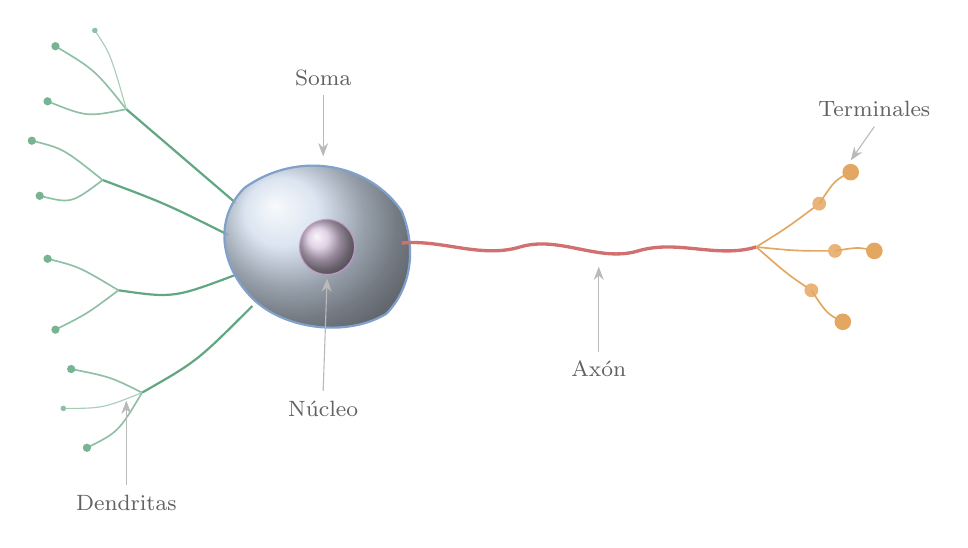
\begin{tikzpicture}[>=Stealth]

% ============================================================
% DENDRITAS (izquierda) — gdlgreen: estructuras, entradas
% ============================================================

% --- Dendrita 1 (superior) ---
\draw[thick, gdlgreen!70] (-1.1, 0.6) .. controls (-1.8, 1.2) .. (-2.5, 1.8);
% Sub-ramas
\draw[semithick, gdlgreen!50] (-2.5, 1.8) .. controls (-2.9, 2.3) .. (-3.4, 2.6);
\fill[gdlgreen!60] (-3.4, 2.6) circle (1.5pt);
\draw[semithick, gdlgreen!50] (-2.5, 1.8) .. controls (-3.0, 1.7) .. (-3.5, 1.9);
\fill[gdlgreen!60] (-3.5, 1.9) circle (1.5pt);
% Ramita extra
\draw[thin, gdlgreen!40] (-2.5, 1.8) .. controls (-2.7, 2.5) .. (-2.9, 2.8);
\fill[gdlgreen!50] (-2.9, 2.8) circle (1pt);

% --- Dendrita 2 (superior-media) ---
\draw[thick, gdlgreen!70] (-1.2, 0.2) .. controls (-2.0, 0.6) .. (-2.8, 0.9);
% Sub-ramas
\draw[semithick, gdlgreen!50] (-2.8, 0.9) .. controls (-3.3, 1.3) .. (-3.7, 1.4);
\fill[gdlgreen!60] (-3.7, 1.4) circle (1.5pt);
\draw[semithick, gdlgreen!50] (-2.8, 0.9) .. controls (-3.2, 0.6) .. (-3.6, 0.7);
\fill[gdlgreen!60] (-3.6, 0.7) circle (1.5pt);

% --- Dendrita 3 (inferior-media) ---
\draw[thick, gdlgreen!70] (-1.1, -0.3) .. controls (-1.9, -0.6) .. (-2.6, -0.5);
% Sub-ramas
\draw[semithick, gdlgreen!50] (-2.6, -0.5) .. controls (-3.1, -0.2) .. (-3.5, -0.1);
\fill[gdlgreen!60] (-3.5, -0.1) circle (1.5pt);
\draw[semithick, gdlgreen!50] (-2.6, -0.5) .. controls (-3.0, -0.8) .. (-3.4, -1.0);
\fill[gdlgreen!60] (-3.4, -1.0) circle (1.5pt);

% --- Dendrita 4 (inferior) ---
\draw[thick, gdlgreen!70] (-0.9, -0.7) .. controls (-1.6, -1.4) .. (-2.3, -1.8);
% Sub-ramas
\draw[semithick, gdlgreen!50] (-2.3, -1.8) .. controls (-2.7, -1.6) .. (-3.2, -1.5);
\fill[gdlgreen!60] (-3.2, -1.5) circle (1.5pt);
\draw[semithick, gdlgreen!50] (-2.3, -1.8) .. controls (-2.6, -2.3) .. (-3.0, -2.5);
\fill[gdlgreen!60] (-3.0, -2.5) circle (1.5pt);
% Ramita extra
\draw[thin, gdlgreen!40] (-2.3, -1.8) .. controls (-2.8, -2.0) .. (-3.3, -2.0);
\fill[gdlgreen!50] (-3.3, -2.0) circle (1pt);

% ============================================================
% SOMA (centro) — gdlblue: espacios, dominios
% ============================================================

% Cuerpo celular: forma orgánica con gradiente 3D
\shade[ball color=gdlblue!25, opacity=0.9]
    (-1.0, 0.8) .. controls (-0.3, 1.3) and (0.6, 1.1) .. (1.0, 0.5)
    .. controls (1.2, 0.0) and (1.1, -0.5) .. (0.8, -0.8)
    .. controls (0.3, -1.1) and (-0.5, -1.0) .. (-0.9, -0.6)
    .. controls (-1.3, -0.2) and (-1.4, 0.4) .. (-1.0, 0.8);
\draw[thick, gdlblue!60]
    (-1.0, 0.8) .. controls (-0.3, 1.3) and (0.6, 1.1) .. (1.0, 0.5)
    .. controls (1.2, 0.0) and (1.1, -0.5) .. (0.8, -0.8)
    .. controls (0.3, -1.1) and (-0.5, -1.0) .. (-0.9, -0.6)
    .. controls (-1.3, -0.2) and (-1.4, 0.4) .. (-1.0, 0.8);

% Núcleo — gdlpurple: acento interno
\shade[ball color=gdlpurple!30] (0.05, 0.05) circle (0.35);
\draw[gdlpurple!50] (0.05, 0.05) circle (0.35);

% ============================================================
% AXÓN (derecha) — gdlred: salida, énfasis
% ============================================================

% Cono axónico (transición soma → axón)
\draw[very thick, gdlred!70]
    (1.0, 0.1) .. controls (1.5, 0.15) and (2.0, -0.1) .. (2.5, 0.05);

% Tronco del axón con ligera ondulación
\draw[very thick, gdlred!70]
    (2.5, 0.05) .. controls (3.0, 0.2) and (3.5, -0.15) .. (4.0, 0.0)
    .. controls (4.5, 0.15) and (5.0, -0.1) .. (5.5, 0.05);

% ============================================================
% TERMINALES AXÓNICOS — gdlorange: transformaciones, mapas
% ============================================================

% Terminal 1 (superior)
\draw[semithick, gdlorange!70] (5.5, 0.05) .. controls (5.9, 0.3) .. (6.3, 0.6);
\fill[gdlorange!60] (6.3, 0.6) circle (2.5pt);
% Botón sináptico
\draw[semithick, gdlorange!70] (6.3, 0.6) .. controls (6.5, 0.9) .. (6.7, 1.0);
\fill[gdlorange!70] (6.7, 1.0) circle (3pt);

% Terminal 2 (medio)
\draw[semithick, gdlorange!70] (5.5, 0.05) .. controls (6.0, 0.0) .. (6.5, 0.0);
\fill[gdlorange!60] (6.5, 0.0) circle (2.5pt);
% Botón sináptico
\draw[semithick, gdlorange!70] (6.5, 0.0) .. controls (6.8, 0.05) .. (7.0, 0.0);
\fill[gdlorange!70] (7.0, 0.0) circle (3pt);

% Terminal 3 (inferior)
\draw[semithick, gdlorange!70] (5.5, 0.05) .. controls (5.9, -0.3) .. (6.2, -0.5);
\fill[gdlorange!60] (6.2, -0.5) circle (2.5pt);
% Botón sináptico
\draw[semithick, gdlorange!70] (6.2, -0.5) .. controls (6.4, -0.8) .. (6.6, -0.9);
\fill[gdlorange!70] (6.6, -0.9) circle (3pt);

% ============================================================
% ETIQUETAS con flechas — gdlgray: auxiliar
% ============================================================

% Etiqueta: Dendritas
\node[font=\footnotesize, text=gdlgray!70!black] (lbl-dend) at (-2.5, -3.2) {Dendritas};
\draw[->, thin, gdlgray!60] (lbl-dend.north) -- (-2.5, -1.9);

% Etiqueta: Soma
\node[font=\footnotesize, text=gdlgray!70!black] (lbl-soma) at (0.0, 2.2) {Soma};
\draw[->, thin, gdlgray!60] (lbl-soma.south) -- (0.0, 1.2);

% Etiqueta: Núcleo
\node[font=\footnotesize, text=gdlgray!70!black] (lbl-nucl) at (0.0, -2.0) {Núcleo};
\draw[->, thin, gdlgray!60] (lbl-nucl.north) -- (0.05, -0.35);

% Etiqueta: Axón
\node[font=\footnotesize, text=gdlgray!70!black] (lbl-axon) at (3.5, -1.5) {Axón};
\draw[->, thin, gdlgray!60] (lbl-axon.north) -- (3.5, -0.2);

% Etiqueta: Terminales sinápticos
\node[font=\footnotesize, text=gdlgray!70!black] (lbl-term) at (7.0, 1.8) {Terminales};
\draw[->, thin, gdlgray!60] (lbl-term.south) -- (6.7, 1.15);

\end{tikzpicture}
\end{document}
